% vim: ts=4 sts=4 sw=4
\documentclass[portuguese, a4paper]{article}
\usepackage[T1]{fontenc}
\usepackage[utf8]{inputenc}
\usepackage{babel}
\usepackage[margin=2.5cm]{geometry}
\usepackage{lmodern}

\usepackage{graphicx}
\graphicspath{ {imagens/} }
\usepackage{wrapfig,lipsum}
\usepackage{bold-extra}
\usepackage{epstopdf}
\usepackage{float}
\usepackage{scalerel}
\usepackage{enumerate}
\usepackage{indentfirst}
\usepackage{mathtools}
\usepackage{amsmath}
\allowdisplaybreaks
\usepackage{amssymb}
\usepackage{listings}
\usepackage{color}
\usepackage{textcomp}
\usepackage{caption}
\usepackage{hyperref}
\hypersetup{
	colorlinks,
	citecolor=black,
	filecolor=black,
	linkcolor=black,
	urlcolor=blue
}

\newcommand\showdiv[1]{\overline{\smash{\hstretch{.5}{)}\mkern-3.2mu\hstretch{.5}{)}}#1}}
\newcommand\ph[1]{\textcolor{white}{#1}}
\newcommand\tu[0]{\textunderscore}

\definecolor{dkgreen}{rgb}{0,0.6,0}
\definecolor{gray}{rgb}{0.5,0.5,0.5}
\definecolor{mauve}{rgb}{0.58,0,0.82}
\definecolor{mygreen}{RGB}{28,172,0} % color values Red, Green, Blue
\definecolor{mylilas}{RGB}{170,55,241}

% ----- Cabeçalho e rodapé -----
\usepackage{fancyhdr}
\pagestyle{fancy}
\fancyhf{}

\renewcommand{\headrulewidth}{1pt}
\renewcommand{\footrulewidth}{0.5pt}

\rhead{2º Trabalho Computacional}
\lhead{Matemática Computacional}
\rfoot{Página \thepage}
\lfoot{\small Engenharia Eletrotécnica e de Computadores - IST}

\usepackage{pdfpages}

\begin{document}
\includepdf[pages={1}]{capa/capa.pdf}

% Secções em números romanos.
\renewcommand{\thesection}{\Roman{section}}
% Subsubsecções no estilo (a), (b), ...
\renewcommand{\thesubsubsection}{(\alph{subsubsection})}

\tableofcontents
\newpage

\section{}
	\subsection{}
	\label{sec:I.1}
	\par
	Resposta no ficheiro \texttt{I/min\tu quad.m}, corrido pelo \emph{script} \texttt{I/1.m}, onde é possível alterar os pontos tabelados, os respetivos pesos e as funções de base.

	\subsection{}
	\par
	Para os dados tabelados:
	\begin{table}[H]
		\centering
		\begin{tabular}{c|c|c|c|c|c|c|c|c|c|c}
			\hline
			$1/e$	& 0.345	& 0.287	& 0.251	& 0.225	& 0.207	& 0.186	& 0.161	& 0.132	& 0.084	& 0.060	\\ \hline
			$s$		& 367	& 311	& 295	& 268	& 253	& 239	& 220	& 213	& 193	& 192	\\ \hline
			$d$		& 17	& 9		& 9		& 7		& 7		& 6		& 6		& 6		& 5		& 5		\\ \hline
		\end{tabular}
		\caption{Dados tabelados.}
	\end{table}

	\par
	Foram obtidas as três funções aproximadoras pedidas, através da função desenvolvida em \ref{sec:I.1}, pelos ficheiros \texttt{I/2\tu i.m}, \texttt{I/2\tu ii.m} e \texttt{I/2\tu iii.m}, corridos no \emph{script} \texttt{I/2.m}.

	\begin{figure}[H]
		\centering
		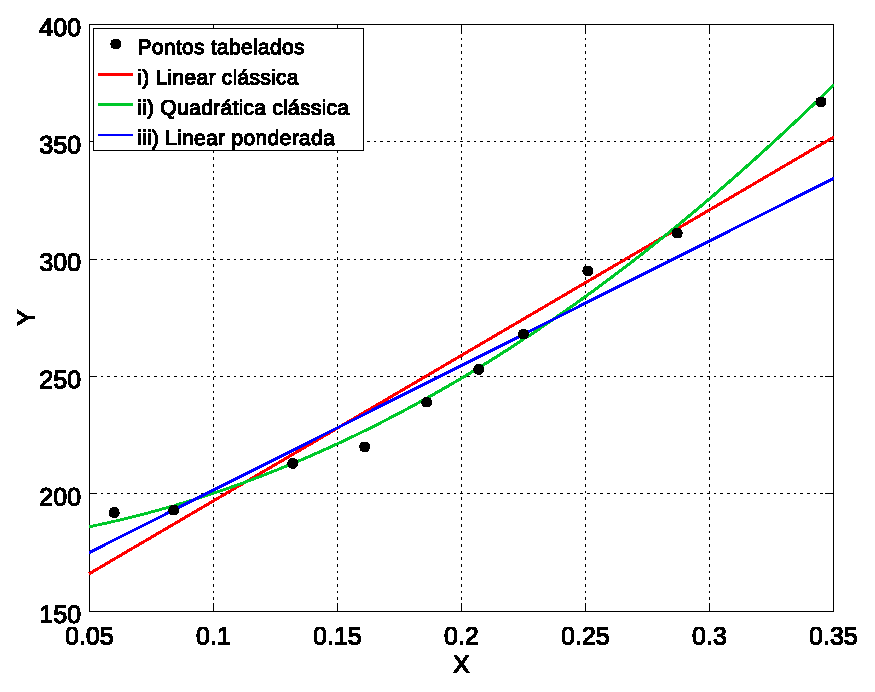
\includegraphics[width=0.80\linewidth]{I_fino}
		\captionsetup{width=0.80\linewidth}
		\caption{Diferentes funções aproximadoras dos pontos tabelados pelo critério dos mínimos quadrados clássico e ponderado.}
	\end{figure}

\newpage

\section{}
	\subsection{}
	\par
	Resposta no ficheiro \texttt{II/simpson.m}, corrido pelo \emph{script} \texttt{II/1.m}, onde é possível alterar o intervalo de integração, o número de subintervalos e a função a integrar.

	\subsection{}
	\subsubsection{}
	\par
	Correndo o programa \texttt{II/2.m}, obtém-se:
	$$F =  1480.56848008215$$

	\subsubsection{}
	\par
	Correndo o programa \texttt{II/2.m}, obtém-se:
	\begin{table}[H]
		\centering
		\begin{tabular}{|c|c|c|c|}
			\hline
			$n$	& $S_n$				& $|F - S_n|$		& $\frac{|F - S_n/2|}{|F - S_n|}$ \\ \hline
			2	& 1219.63999486000	& 260.92848522216	& -					\\ \hline
			4	& 1426.86928844946	& 53.69919163269	& 4.85907659480		\\ \hline
			8	& 1473.14779849473	& 7.42068158743		& 7.23642309672		\\ \hline
			16	& 1479.85678890922	& 0.71169117293		& 10.42682819413	\\ \hline
			32	& 1480.51545319880	& 0.05302688335		& 13.42132759730	\\ \hline
			64	& 1480.56497529815	& 0.00350478401		& 15.12985771736	\\ \hline
			128	& 1480.56825767195	& 0.00022241020		& 15.75819799559	\\ \hline
			256	& 1480.56846613061	& 0.00001395154		& 15.94162455869	\\ \hline
			512	& 1480.56847921284	& 0.00000086931		& 16.04897985126	\\ \hline
		\end{tabular}
		\caption{Comparação dos erros da regra de Simpson para vários valores de N.}
	\end{table}

	% TODO: comentar os erros
	% a majoração do erro depende de N quarticamente, por isso,
	% se N duplicar, o erro cai para 1/16.

\end{document}
